% arara: pdflatex
% arara: nomencl
% arara: pdflatex
% !TEX TS-program = arara
\documentclass[11pt]{article}
\usepackage[margin=1.0in]{geometry}         
\geometry{letterpaper}    
\usepackage{graphicx}
\usepackage{amssymb}
\usepackage{amsmath}
\usepackage{epstopdf}
\usepackage[]{nomencl}
\usepackage{float} 
\usepackage{listings}
\usepackage{color}
\usepackage{hyperref}
\makenomenclature
\DeclareGraphicsRule{.tif}{png}{.png}{`convert #1 `dirname #1`/`basename #1 .tif`.png}
\DeclareGraphicsRule{.gif}{png}{.png}{`convert #1 `dirname #1`/`basename #1 .gif`.png}

%%% START OF MODIFIABLE CODE %%%

\title{Use and Application of the neuralnet Package in R}
\author{Mridu Nanda \\ Nikhil Milind \\ Alan York \\ North Carolina School of Science and Math}

%%% LEAVE THIS STUFF ALONE %%%

\begin{document}
\maketitle

%%% CONTINUING MODIFIABLE STUFF %%%

\section{Mr. Gotwals Sample}

\nomenclature{Glossary term:}{Definition}

In this part, describe the scientific background for this particular project.  You can also describe the specific R skill(s) that will be learned with this project.  \cite{boyce}

 Look at the picture in Figure \ref{fig:model}. 

Here is how to do a list:

\begin{enumerate}
\item typical commands such as clear-all, reset-ticks,  ask, set-default-shape, create-\emph{breeds}, etc.
\item  breed
\item globals
\item set
\item heading
\item xcor and ycor (turtles)
\item pxcor and pycor (patches)
\end{enumerate}

Here is how to do graphics:

\begin{figure}[H] %  the "H" means put it where you put this code....but that doesn't always work!
   \centering
      \caption{Model Settings window}
   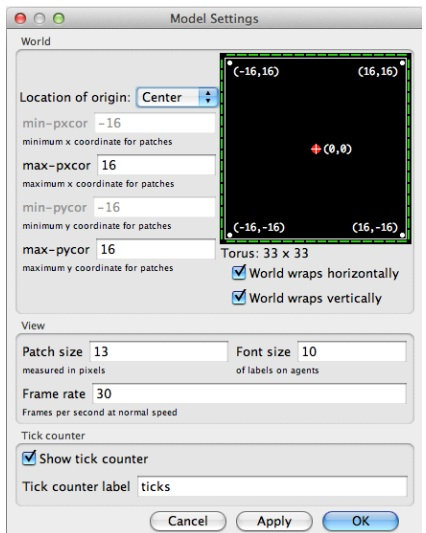
\includegraphics[scale=0.5]{model.jpg} 
   \label{fig:model}
\end{figure}

\section{Objectives of the Case Study}

Here is where you describe what the assignment is and what the student(s) is/are expected to do. 

\subsection{Objective 1}

blah blah blah

\subsection{Objective 2}

Blah blah blah
 

\section{Building the Model}

In this section, describe how the student(s) might approach building this model.  Include sample graphics (what the student should get if the code is done right), code snippets as appropriate, etc. 

 \subsection{Programming Hints}
 
If appropriate, put some suggestions or hints as to what to do.
 
\section{Deliverable}

Describe what the student(s) should submit as the final delverable.

\section{Teaching Code}

This is where you put your sample code that the instructor will use to teach the skills necessary to complete this lab.
You should also put any notes, teaching suggestions, etc. in this space!


\begin{verbatim}
 # Robert Gotwals
# July 19, 2016
# hyper.R script
# this script analyzes BP data
#
# clean up and set directory
rm(list=ls())
setwd("/Users/gotwals/desktop/RFolder")
#
# load the QTL library
library(qtl)
# load myfunctions.R file
source("myfunctions.R")
#
\end{figure}
\end{verbatim}

\section{Example Student Code}

This is where you put code that a student would write (in other words, a \textbf{key}.

\begin{verbatim}
 # Robert Gotwals
# July 19, 2016
# hyper.R script
# this script analyzes BP data
#
# clean up and set directory
rm(list=ls())
setwd("/Users/gotwals/desktop/RFolder")
#
# load the QTL library
library(qtl)
# load myfunctions.R file
source("myfunctions.R")
#
\end{figure}
\end{verbatim}

\section{Further Readings}

Suggest other things that the student might read.

\begin{thebibliography}{99}

\bibitem{nielsen}
Michael A. Nielsen, "Neural Networks and Deep Learning," Determination Press, 2015

\end{thebibliography}


\printnomenclature

\end{document}  